\documentclass{article}
\usepackage[utf8]{inputenc}
\usepackage{amsmath}
\usepackage{amsfonts}
\usepackage{amssymb}
\usepackage{tikz}
\usetikzlibrary{positioning, arrows.meta, automata}

\title{Ejercicios Capítulo 2 - Cadenas de Markov}
\author{Apuntes de Clase}
\date{\today}

\begin{document}

\maketitle

\section{Problema}

Un barbero corta el pelo a tres personas por hora y los clientes llegan a su tienda según un proceso de Poisson con intensidad de 2 por hora.  
Los clientes no entran si las dos sillas de espera están siendo usadas.  
¿Qué fracción del tiempo la barbería estará llena?

\textbf{Solución:} 

Sea $X_t$ el número de personas en la barbería en el tiempo $t$.

\begin{center}
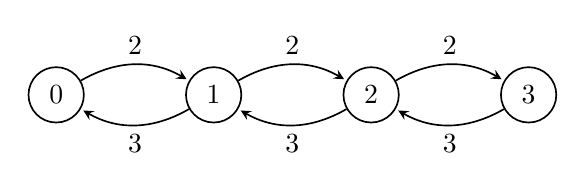
\begin{tikzpicture}[scale=1,->,>=stealth,shorten >=1pt,auto,node distance=2cm,semithick]
\tikzstyle{every state}=[fill=white,draw=black,text=black,minimum size=20pt]
\node[state] (A) {0};
\node[state] (B) [right of=A] {1};
\node[state] (C) [right of=B] {2};
\node[state] (D) [right of=C] {3};

\path
(A) edge[bend left] node{$2$} (B)
(B) edge[bend left] node{$3$} (A)
(B) edge[bend left] node{$2$} (C)
(C) edge[bend left] node{$3$} (B)
(C) edge[bend left] node{$2$} (D)
(D) edge[bend left] node{$3$} (C);
\end{tikzpicture}
\end{center}

El proceso $(X_t)$ es un proceso de nacimiento y muerte con estados $\{0, 1, 2, 3\}$.

Las tasas de transición son:
\begin{align*}
q(i, i+1) &= 2, \quad i = 0, 1, 2 \\
q(i, i-1) &= 3, \quad i = 1, 2, 3
\end{align*}

Para encontrar las probabilidades de estado estacionario, usamos las ecuaciones de balance detallado:
\begin{align*}
q(i, i-1) \Pi_i &= q(i-1, i) \Pi_{i-1} \\
q(x, y) \Pi_x &= q(y, x) \Pi_y
\end{align*}

Calculando las probabilidades en términos de $\Pi_0$:
\begin{align*}
\Pi_1 &= \frac{\lambda_0}{\mu_1} \Pi_0 = \frac{2}{3} \Pi_0 \\
\Pi_2 &= \frac{\lambda_1}{\mu_2} \Pi_1 = \frac{2}{3} \Pi_1 = \left(\frac{2}{3}\right)^2 \Pi_0 \\
\Pi_3 &= \frac{\lambda_2}{\mu_3} \Pi_2 = \frac{2}{3} \Pi_2 = \left(\frac{2}{3}\right)^3 \Pi_0
\end{align*}

Aplicando la condición de normalización:
\begin{align*}
\sum_{i=0}^{3} \Pi_i &= 1 \\
\Pi_0 + \frac{2}{3}\Pi_0 + \left(\frac{2}{3}\right)^2\Pi_0 + \left(\frac{2}{3}\right)^3\Pi_0 &= 1
\end{align*}

Resolviendo para $\Pi_0$:
\begin{align*}
\Pi_0 &= \frac{1}{1 + \sum_{k=1}^{3} \left(\frac{2}{3}\right)^k} \\
\Pi_0 &= \frac{27}{65}
\end{align*}

Por lo tanto, las probabilidades de estado estacionario son:
\begin{align*}
\Pi_0 &= \frac{27}{65} \\
\Pi_1 &= \frac{2}{3} \times \frac{27}{65} = \frac{18}{65} \\
\Pi_2 &= \frac{4}{9} \times \frac{27}{65} = \frac{12}{65} \\
\Pi_3 &= \frac{8}{27} \times \frac{27}{65} = \frac{8}{65}
\end{align*}

\textbf{¿Cuál es la cantidad de personas que no entran?}

Esto se refiere a la probabilidad de que un cliente que llega no pueda entrar porque la barbería está llena (estado 3).

\begin{align*}
P(\text{entra}) &= 1 - \Pi_3 = 1 - \frac{8}{65} = \frac{57}{65} \\
P(\text{no entra}) &= \Pi_3 = \frac{8}{65}
\end{align*}

Consideramos las llegadas de clientes y las clasificamos en dos tipos:

\begin{center}
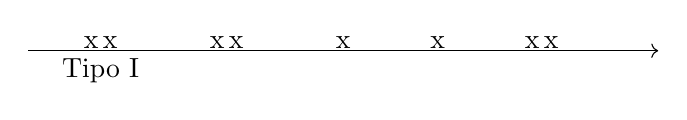
\begin{tikzpicture}[x=0.8cm, y=0.5cm]
    % Línea con flecha
    \draw[->] (0,0) -- (10,0);
    % Marcas x
    \node at (1,0.2) {x};
    \node at (1.3,0.2) {x};
    \node at (3,0.2) {x};
    \node at (3.3,0.2) {x};
    \node at (5,0.2) {x};
    \node at (6.5,0.2) {x};
    \node at (8,0.2) {x};
    \node at (8.3,0.2) {x};
    % Etiquetas
    \node at (1.15,-0.5) {Tipo I};
\end{tikzpicture}
\end{center}

Las tasas de llegada para cada tipo de cliente, modeladas como procesos de Poisson, son:
\begin{align*}
\text{Tipo I (clientes que entran)} &\sim \text{PP}\left(\lambda \times P(\text{entra})\right) = \text{PP}\left(2 \times \left(1 - \frac{8}{65}\right)\right) \\
\text{Tipo II (clientes que no entran)} &\sim \text{PP}\left(\lambda \times P(\text{no entra})\right) = \text{PP}\left(2 \times \frac{8}{65}\right)
\end{align*}

La fracción del tiempo que la barbería estará llena (estado 3) es $\Pi_3 = \frac{8}{65} \approx 0.123$ o $12.3\%$.

\section{Problema de las Máquinas}

Una fábrica tiene tres máquinas en uso. Suponga que una máquina funciona bien con tiempo exponencial con media de 60 días entre averías. Cada avería necesita un tiempo exponencial con media de 4 días para ser reparada. Solo hay una persona reparando las máquinas. ¿Cuál es la proporción de días, a largo plazo, que las tres máquinas estarán trabajando?

\textbf{Solución:}

Sea $X_t$ el número de máquinas trabajando.

Cálculo de la tasa de falla: $\frac{1}{\lambda} = 60 \Rightarrow \lambda = \frac{1}{60}$

\begin{center}
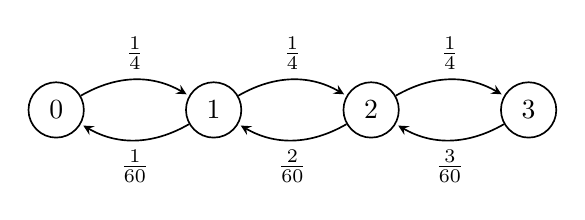
\begin{tikzpicture}[scale=1,->,>=stealth,shorten >=1pt,auto,node distance=2cm,semithick]
\tikzstyle{every state}=[fill=white,draw=black,text=black,minimum size=20pt]
\node[state] (A) {0};
\node[state] (B) [right of=A] {1};
\node[state] (C) [right of=B] {2};
\node[state] (D) [right of=C] {3};

\path
(A) edge[bend left] node{$\frac{1}{4}$} (B)
(B) edge[bend left] node{$\frac{1}{60}$} (A)
(B) edge[bend left] node{$\frac{1}{4}$} (C)
(C) edge[bend left] node{$\frac{2}{60}$} (B)
(C) edge[bend left] node{$\frac{1}{4}$} (D)
(D) edge[bend left] node{$\frac{3}{60}$} (C);
\end{tikzpicture}
\end{center}

$X_t$ es un proceso de nacimiento y muerte:

\begin{align*}
\lambda_i &= q(i,i+1) = \frac{1}{4} \quad i=0,1,2 \\
\mu_i &= q(i,i-1) = \frac{i}{60} \quad i=1,2,3
\end{align*}

\begin{center}
\fbox{$\Pi_k = \frac{\lambda_{k-1}}{\mu_k} \Pi_{k-1}$}
\end{center}

\begin{align*}
\Pi_1 &= \frac{\lambda_0}{\mu_1} \Pi_0 = \frac{1/4}{1/60} \Pi_0 = \frac{60}{4} \Pi_0 \\
\Pi_2 &= \frac{\lambda_1}{\mu_2} \Pi_1 = \frac{1/4}{2/60} \Pi_1 = \frac{60}{8} \Pi_1 \\
\Pi_3 &= \frac{\lambda_2}{\mu_3} \Pi_2 = \frac{1/4}{3/60} \Pi_2 = \frac{60}{12} \Pi_2
\end{align*}

Desarrollando las expresiones en términos de $\Pi_0$:
\begin{align*}
\Pi_1 &= \frac{60}{4} \Pi_0 \\
\Pi_2 &= \frac{60^2}{4 \times 8} \Pi_0 \\
\Pi_3 &= \frac{60^3}{4 \times 8 \times 12} \Pi_0
\end{align*}

Aplicando la condición de normalización:
\begin{align*}
\Pi_0 + \Pi_1 + \Pi_2 + \Pi_3 &= 1 \\
\Pi_0 + \frac{60}{4}\Pi_0 + \frac{60^2}{4 \times 8}\Pi_0 + \frac{60^3}{4 \times 8 \times 12}\Pi_0 &= 1 \\
\Pi_0 \left(1 + \frac{60}{4} + \frac{60^2}{4 \times 8} + \frac{60^3}{4 \times 8 \times 12}\right) &= 1 \\
\Pi_0 (1 + 15 + 112.5 + 562.5) &= 1 \\
\Pi_0 \times 691 &= 1 \\
\Pi_0 &= \frac{1}{691}
\end{align*}

Por lo tanto, las probabilidades de estado estacionario son:
\begin{align*}
\Pi_0 &= \frac{1}{691} \\
\Pi_1 &= \frac{60}{4 \times 691} = \frac{15}{691} \\
\Pi_2 &= \frac{60^2}{4 \times 8 \times 691} = \frac{225}{1382} \\
\Pi_3 &= \frac{60^3}{4 \times 8 \times 12 \times 691} = \frac{1125}{1382}
\end{align*}

\section{Problema de la Tienda}

En una tienda los clientes llegan según un proceso de Poisson con tasa 1 por hora y cada cliente es atendido un tiempo exponencial con tasa de 2 por hora. ¿Cuál es la proporción del tiempo, a largo plazo, que la tienda estará vacía?

\textbf{Solución:}

Sea $X_t$ el número de clientes en la tienda al tiempo $t$.

\begin{center}
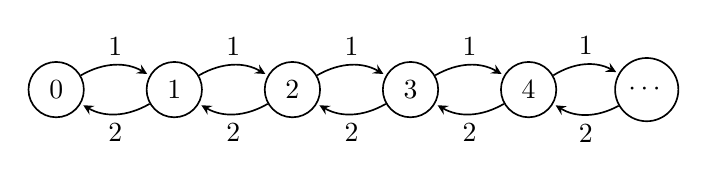
\begin{tikzpicture}[scale=1,->,>=stealth,shorten >=1pt,auto,node distance=1.5cm,semithick]
\tikzstyle{every state}=[fill=white,draw=black,text=black,minimum size=20pt]
\node[state] (A) {0};
\node[state] (B) [right of=A] {1};
\node[state] (C) [right of=B] {2};
\node[state] (D) [right of=C] {3};
\node[state] (E) [right of=D] {4};
\node[state] (F) [right of=E] {$\cdots$};

\path
(A) edge[bend left] node{$1$} (B)
(B) edge[bend left] node{$2$} (A)
(B) edge[bend left] node{$1$} (C)
(C) edge[bend left] node{$2$} (B)
(C) edge[bend left] node{$1$} (D)
(D) edge[bend left] node{$2$} (C)
(D) edge[bend left] node{$1$} (E)
(E) edge[bend left] node{$2$} (D)
(E) edge[bend left] node{$1$} (F)
(F) edge[bend left] node{$2$} (E);
\end{tikzpicture}
\end{center}

$X_t$ es un proceso de nacimiento y muerte:

\begin{align*}
q(i, i+1) &= 1 \\
q(i, i-1) &= 2
\end{align*}

Calculando las probabilidades de estado estacionario en términos de $\Pi_0$:
\begin{align*}
\Pi_1 &= \frac{\lambda_0}{\mu_1} \Pi_0 = \frac{1}{2} \Pi_0 \\
\Pi_2 &= \frac{\lambda_0 \lambda_1}{\mu_1 \mu_2} \Pi_0 = \left(\frac{1}{2}\right)^2 \Pi_0 \\
\Pi_3 &= \frac{\lambda_0 \lambda_1 \lambda_2}{\mu_1 \mu_2 \mu_3} \Pi_0 = \left(\frac{1}{2}\right)^3 \Pi_0 \\
&\vdots \\
\Pi_n &= \frac{\lambda_0 \lambda_1 \dots \lambda_{n-1}}{\mu_1 \mu_2 \dots \mu_n} \Pi_0 = \left(\frac{1}{2}\right)^n \Pi_0
\end{align*}

Aplicando la condición de normalización:
\begin{align*}
\sum_{i=0}^{\infty} \Pi_i &= 1 \\
\sum_{i=0}^{\infty} \left(\frac{1}{2}\right)^i \Pi_0 &= 1 \\
\Pi_0 \sum_{i=0}^{\infty} \left(\frac{1}{2}\right)^i &= 1 \\
\Pi_0 \times 2 &= 1 \\
\Rightarrow \Pi_0 &= \frac{1}{2}
\end{align*}

Por lo tanto, la probabilidad de estado estacionario para el estado $n$ es:
\begin{align*}
\Pi_n &= \frac{1}{2} \left(\frac{1}{2}\right)^n
\end{align*}

La proporción del tiempo que la tienda estará vacía es $\Pi_0 = \frac{1}{2}$.

\end{document}
